\section{Adding buildings}
\label{sec:addingbuildings}
As a player you may want to add buildings to the world. In this section we will explain how a player can add buildings and how we have implemented this feature.

\subsection{Controls and feedback}
Buildings can be spawned via the building panel (see \cref{fig:building-panel}). When the player clicks on the building that he/she wishes to spawn, or presses the key that belongs to the building (displayed in the top left corner of the building in the building panel), a slightly transparent texture of the building appears at the mouse position. When the player hovers the mouse over another static entity, the texture gets a red border. This will notify the player that the building cannot be placed at that current mouse position. If the player decides not to place a building after all, the action can be cancelled by pressing the escape key. More on this subject is described in \cref{AbortPlacingBuilding}. When the player is satisfied with the position to place the building on, it can be placed by clicking the left mouse button. 

\subsection{Building panel}
The building panel, as displayed in \cref{fig:building-panel}, iterates over the buildings\_with\_textures enum, and for each entry it adds a UnitPanel to the Building Panel. UnitPanels are used for the EntityPanel (see \ref{EntityPanel}) as well as the Building Panel. These UnitPanels render an image, and contain objects of whatever it renders (buildings or entities). Unit panels are highlighted in \cref{fig:unit-panel}.

A mouse handler of which a diagram is shown in \cref{fig:mousehandlerbuildingpanel}, or the key event handler takes care of actually starting the process of positioning and placing a building. The shortcut keys to start this process are located at the top left corner of the unit panel, as shown in \cref{fig:building-shortcuts}.

\subsection{States}
We are using the state pattern during positioning and placing buildings, because this pattern makes it easy to extend the behaviour of the player or entity, which can be different each state.\\
When a player clicks on a building in the building panel, the mouse handler will look at the player its current state. If the player is already in the ChoosingBuildingPosition state, then the player wants to 
set the current mouse position as the final position of the building, and the player its state will change to the  PlacingBuilding state.\\
If the player is not in the ChoosingBuildingState state, the mouse  handler will call the method 
choosing\_building\_position, which belongs to the BuildingManager. The building manager is responsible for creating the building entity, together with the BuildingFactory.
When the entity is created, it will be added to the world so this object will be rendered.
The BuildingManager will also set the positioning\_object variable of the player, so the player can keep track of the building it is positioning from now on. After all this is done, the state of the player will be changed to ChoosingBuildingPosition.
A state machine diagram explaining state transitions can be found in \cref{fig:statediagram-addingbuildings} and a class diagram with relevant methods, associations and variables can be found in \cref{fig:classdiagram-addingbuildings}.

\begin{figure}[H]
    \centering
    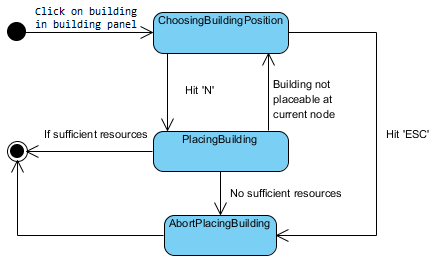
\includegraphics{res/adding-buildings/States-StateDiagram.png}
    \caption{Adding buildings state diagram.}\label{fig:statediagram-addingbuildings}
\end{figure}

\subsubsection{ChoosingBuildingPosition}
At entering this state, the texture its opacity will be set to 70\%. We have chosen to do so, because this will make clear which objects are already placed and which objects are not placed by the player yet.\\
During the execute method of this state the mouse position of the player will be tracked. If the mouse position has changed, the GraphManager will be consumed to get the nearest node in relation to the mouse position. If there is another static entity on that node, we want to inform the player by changing the entity its texture by adding a red border.

\subsubsection{PlacingBuilding}
The PlacingBuilding state will be entered when the player clicks the left mouse button in the game world while it is in the ChoosingBuildingPosition state. This state only has logic in its enter method, because it needs to make one decision: can the building be positioned at this position or not.\\
If the building cannot be positioned at the node, the state will be changed back to ChoosingBuildingPosition, to give the user another chance to find a good spot for the building. If the building can be placed at the node and the player has enough resources to cover the costs for a building, the entity will be added to the building array of the player and to the building array of the BuildingManager. The costs of the building will be subtracted from the player its gathered resources. The opacity will also be set to 0\%. The positioning\_object variable kept by the player object will be cleared, just like the current state of the user.

\subsubsection{AbortPlacingBuilding} \label{AbortPlacingBuilding}
This state will be entered when a player is in the ChoosingBuildingPosition state and it hits the 'ESC' key. It also will be entered after a player enters the PlacingBuilding and it has not enough resources to place the building. The method only has logic in the enter method and it fires the remove\_building() method from the BuildingFactory. 

\begin{figure}[!htb]
    \centering
    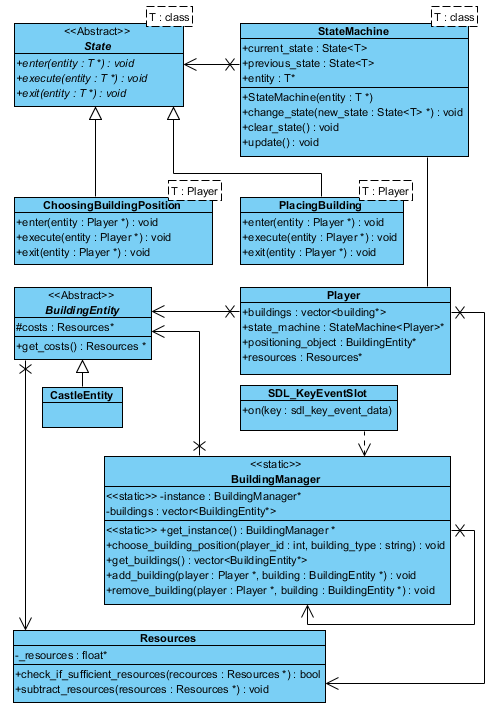
\includegraphics{res/adding-buildings/States-ClassDiagram.png}
    \caption{Adding buildings class diagram.}\label{fig:classdiagram-addingbuildings}
\end{figure}
\clearpage



